\chapter{The CMS Detector}\label{sec:detectors}

Since the discovery of the neutron in 30s, humanity's aspiration to understand the most fundamental constituents and laws of the physics have only accelerated.
Discovery of pions, Kaons, and other hadrons from the cosmic rays in 40s, 50s led to understanding of substructure of those particles with Eightfole way of Gell-Mann.
Deep inelastic scattering performed in 60s by the Stanford Linear Accelerator Center (SLAC) confirmed existence of "partons" or "quarks", substructure of those particles.
Observance of J-psi and Upsilon mesons in SLAC and MIT put the third generation fermions in the collection of particles.
Gargamelle bubble chamber in CERN succeeded in detection of muon neutrinos, postulated by Pauli in 30s from the beta decay experiment.
CERN's UA1 and UA2 in 80s confirmed existence of first particles in the electroweak scale, namely the W and Z bosons.
Fermilab's CDF and D0 in 90s confirmed existence of the top quark, the heaviest particle in the SM.
All these discoveries of the most fundamental particles of the universe happened within a half-century.
As much as we appreciate the predecessor physicists for the phenomenal analytic and statistical works, we need to appreciate the evolution of the experimental apparatus as well.
Although simple design of bubble chamber or detection of cosmic rays is still a helpful insight for particle physics research, physicists wanted to create the cosmic and very early phase of the universe on our terra.
Progress from the linear accelerator to TeV scale circular high energy accelerator was achieved by physicists, engineers, and others.
Its pinnacle came with construction fo the LHC, situated in CERN, the home of UA(1-5). 



\section{The LHC and the CMS}
The LHC is the world's largest and highest energy particle collider.
The LHC was built for a decade from 1998 to 2008. 
The construction was completed in collaboration with 100 countries and 10000 scientists around the globe, demostrating the ethos of global cooperation of the physics community and its majestic scale. 
The LHC construction, which costed 5 billion us dollars for its construction , costs 5.5 billion dollars per year for its electric and computing power consumption \cite{LHCweb}.
The LHC is built in a tunnel 328 feet underground at CERN, on the Franco-Swiss border near Annecy, France and  Geneva, Switzerland.
The LHC shoots bunches of protons and lead ions near the speed of light, enabled by the 27 km ring of superconducting magnets with a number of accelerating apparati.
One can infer the LHC name's origin, given that it's 27km long, shoots hadrons of protons, and collide them each other at 0.9997 fraction of the speed of light.

CERN is an acclerator complex, which includes succession of machines with increasingly higher energies. 
\begin{figure}[h!]
	\caption{Picture of the CERN complex \cite{CERN}}
  \label{fig:CERN}
  \centering
  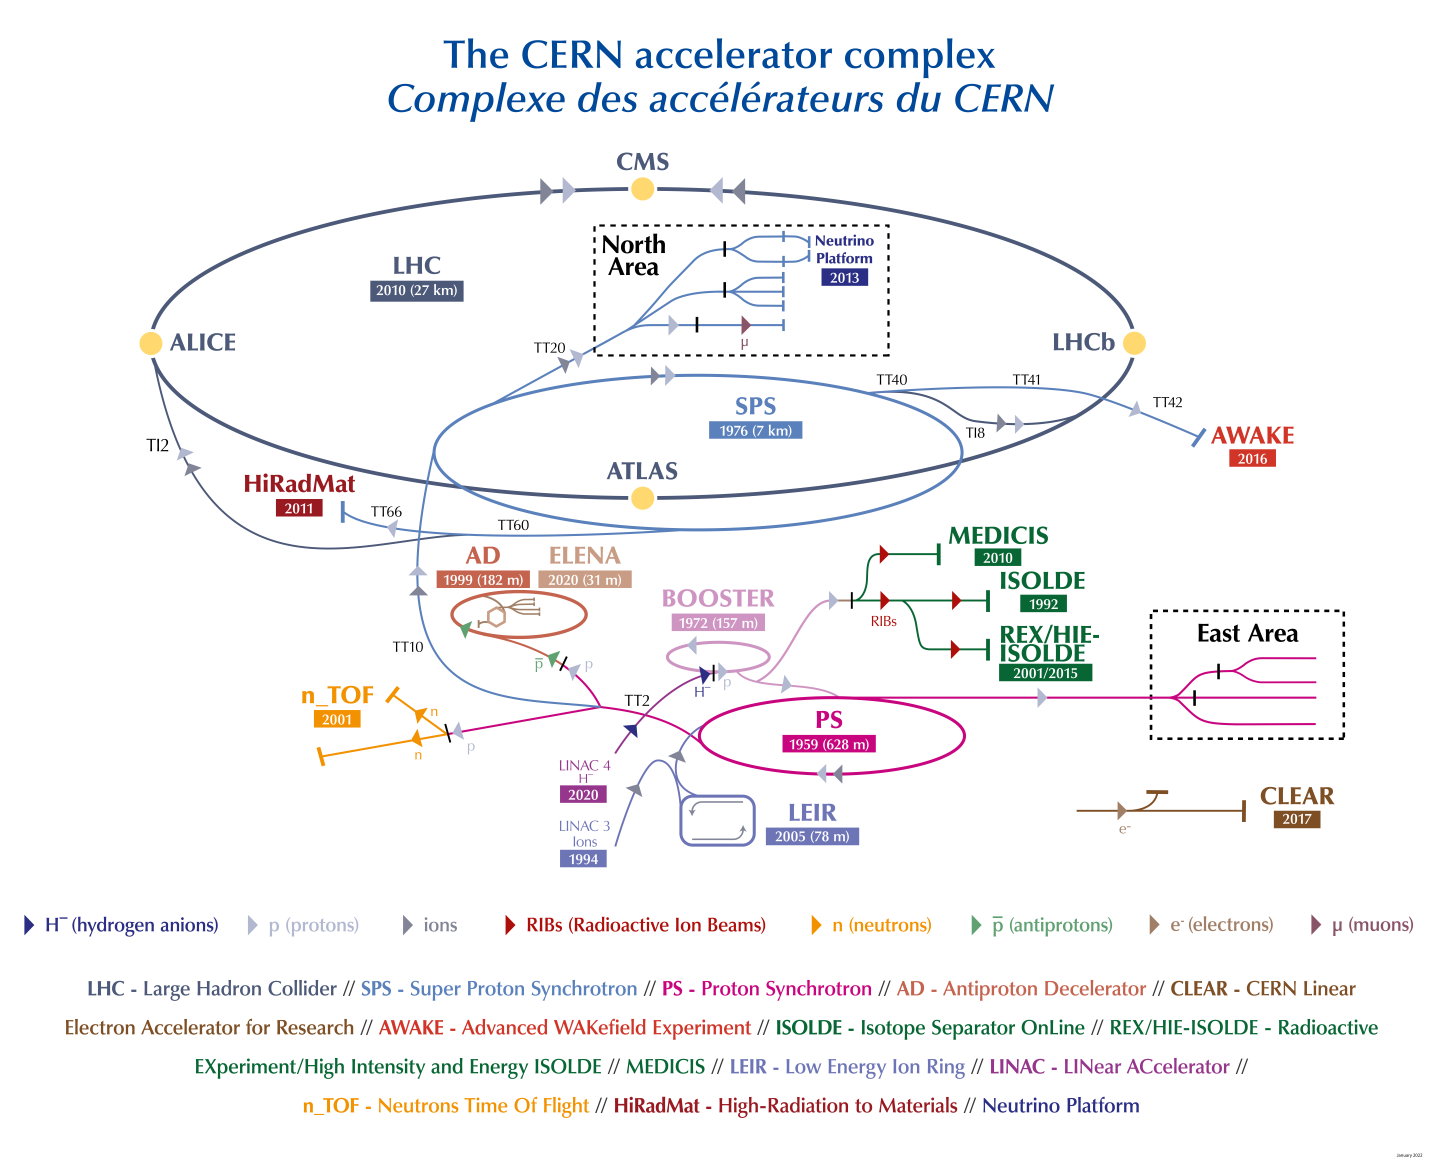
\includegraphics[width=0.9\linewidth]{figs/LHC.png}
\end{figure}
Each machine accelerates a beam of particles to a threshold of desired energy, and injects the beam into the next machine in the chain. 
The next machine brings the beam to an even higher energy and repeats the cycle until the entering the LHC. 
The LHC is the last element of this chain, in which the beams reach their highest energies.
The LHC is cooled to 1.9K and maintained at ultrahigh vacuum status.

The goal of LHC was to discover the last remaining piece of the SM, the Higgs boson.
The LHC already succeeded in its primary goal, with discovery of the Higgs boson bo the CMS and ATLAS in July 4th, 2012.
However, the LHC's goal does not stop there. 
As mentioned in \ref{sec:theory}, there still exists several unanswered questions in high energy physics.
LHC wants to address them. It wants to discover the SUSY particles, dark matters, and other exotic particles to help us better understand the most fundamental nature of the universe.

In order to tackle these issues more efficienctly, there are 4 main detectors in the LHC: Compact Muon Solenoid (CMS), A Toroidal LHC Apparatus (ATLAS), A Large Ion Collider Experiment (ALICE), and LHCb.
CMS and ATLAS are general purpose colliders. They were used for the discovery of the Higgs Boson in 2012. They are used for an entire range of the high energy physics, investigating the SUSY particles to dark matter to precision QCD to Lepton Universality.
ALICE is a lead-lead collider, targeting to study a phase of matter called the Quark-Gluon Plasma (QGP). Study of QGP helps us better understand quarks and gluons behavior when they esacape the confinement of the QCD.
Similar research is done in Brookhaven National Laboratory's Pioneering High Energy Nuclear Interaction eXperiment (BNL's PHENIX).
LHCb is a b-factory. It wants to test or challenge "Lepton Universality", claiming that interaction between leptons and a gauge boson measures the same for each lepton. 
Similar research is done in BaBar of SLAC and BelleII of KoEnerugi Kasokuki kenkyu kiko (KEK).
The analysis of this dissertation entirely derives from data obtained in the CMS.
Following subsections detail parts and functions of each part of the CMS.
\begin{figure}[h!]
	\caption{Picture of the CMS viewed from the beam direction \cite{det}}
  \label{fig:cms}
  \centering
  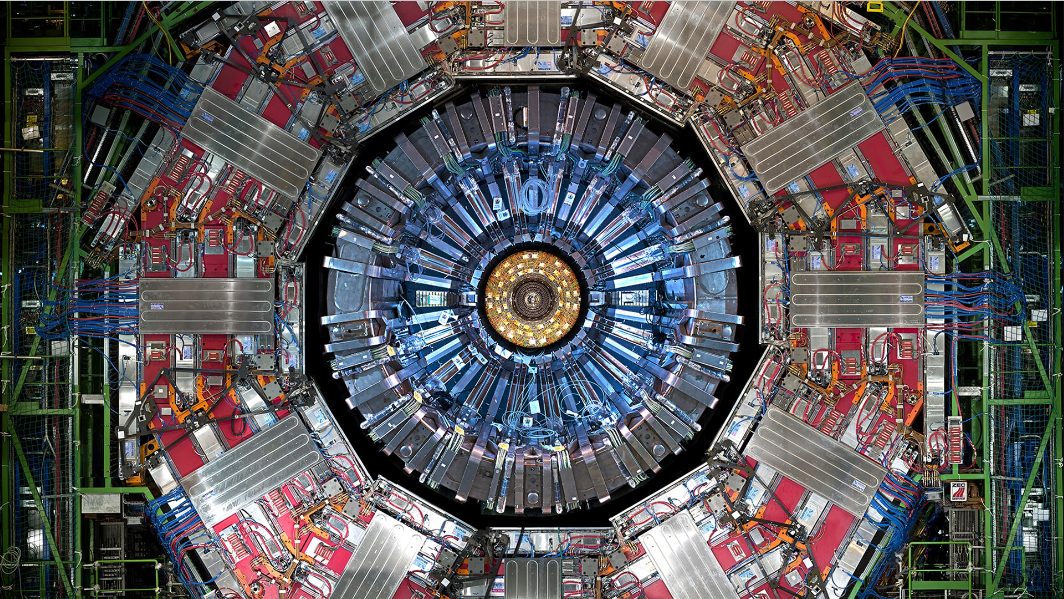
\includegraphics[width=0.9\linewidth]{figs/cms.png}
\end{figure}

The CMS consists of 5 main parts: the tracker, the electromagnectic calorimeter (ECAL), the hadronic calorimeter, the superconducting magnet and the Muon chamber.
\begin{figure}[h!]
	\caption{Cartoon of the CMS with its subpart annotated \cite{xsec}}
  \label{fig:CMS}
  \centering
  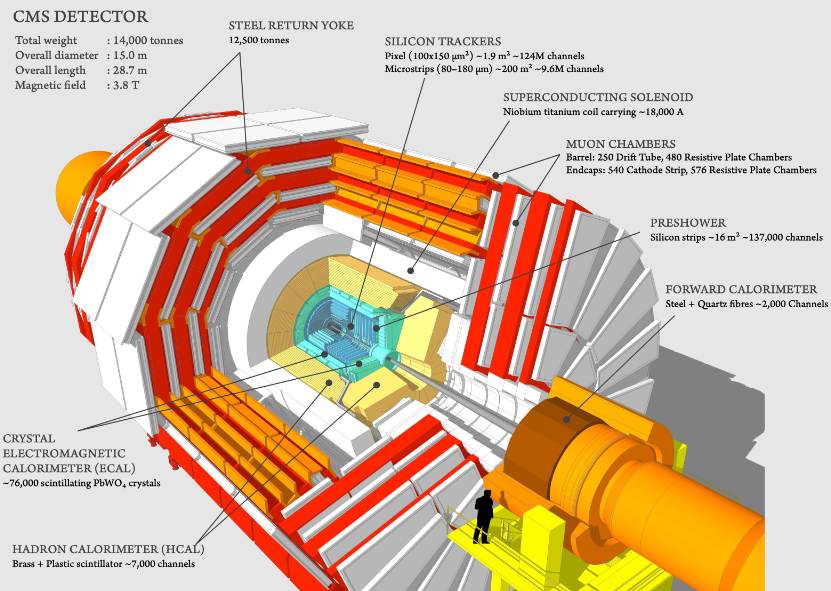
\includegraphics[width=0.87\linewidth]{figs/CMS.png}
\end{figure}
We will review each part's hardware information and its role in terms of the entire CMS.
The order of review is identical as a particle's trajectory from the beamspot as in \ref{fig:cmsxsec}, except that the tracker is placed at the end for its connection to my analysis' trigger strategy.
\begin{figure}[h!]
  \caption{Cross-section of the CMS detector as a particle traverses through the apparatus \cite{xsec}}
  \label{fig:cmsxsec}
  \centering
  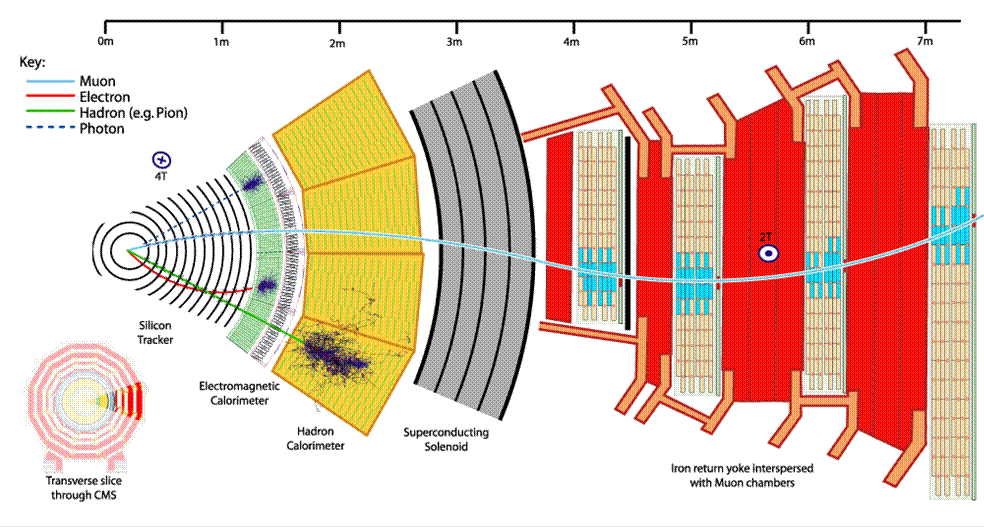
\includegraphics[width=0.87\linewidth]{figs/cmsxsec.png}
\end{figure}
\subsection{Calorimetry}
\subsubsection{ECAL of the CMS}
\begin{figure}[h!]
  \caption{Schematic view of the ECAL. \cite{ecal}}
  \label{fig:ECAL}
  \centering
  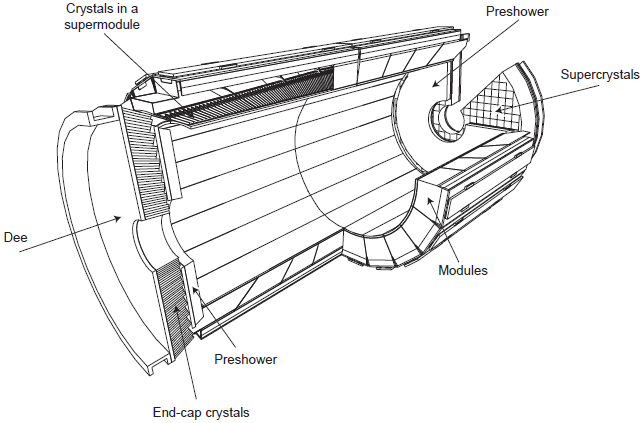
\includegraphics[width=0.87\linewidth]{figs/ECAL.png}
\end{figure}
Electron and photon energies are measured in the ECAL with high precision. 
CMS has a compact scintillating crystal calorimeter with excellent performance for energy resolution.
The ECAL consists of 75,000 lead-tungstate (PbWO4) crystals with coverage in pseudorapidity upto 3.0. As photons and electrons shower through the crystals, their radiation light is detected by silicon avalanche photodiodes (APDs) in the barrel and vacuum phototriodes (VPTs) in the endcap.
ECAL distinguises photons from electron based on the the energy dispersion on the i$\eta$-i$\phi$ map as photon's energy is deposited into a wider area.
ECAL can also distinguish $\pi^{0}$, which decay into 2 photons, from photons originating from the hard scattering.
ECAL's preshower system installed in the front of the endcap is used for $\pi^{0}$ rejection and the detection of photons. 

\subsubsection{HCAL of the CMS}
\begin{figure}[h!]
  \caption{Cross-section of the HCAL in the CMS detector. It shows the Barrel, endcap, front, and outside portion. \cite{hcal}}
  \label{fig:HCAL}
  \centering
  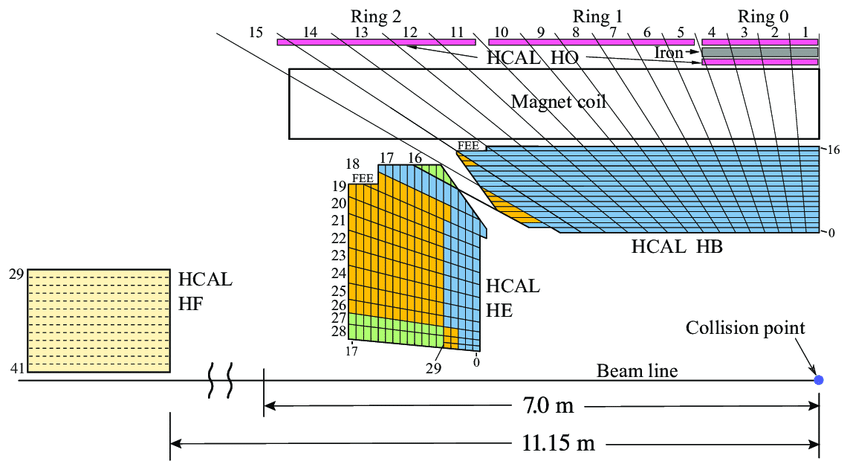
\includegraphics[width=0.87\linewidth]{figs/HCAL.png}
\end{figure}
The ECAL is surrounded by brass/scintillator sampling Hadron Calorimeter (HCAL) with pseudorapidity upto 3.0.
Strongly interacting SM particles, such as quarks, gluons, deposit their energy into the HCAL.
These particles are in form on hadrons, due to color confinement of QCD, and hadrons' shower is more messy than electromagnetically interacting particles.
We indentify these strongly interacting particles, as a jet, which is a narrow cone of hadrons and other particles produced by the hadronization of a quark or gluon.
HCAL plays an important role in the identification and measurement of neutrinos by measuring the energy and direction of jets.
Since the initial momentum in the transverse plane, which is a plane perpendicular to the beam(z) direction, is 0, the final transeverse momentum is also equal to 0.
If the final transverse momentum is not equal to 0, or there is missing transverse energy (MET), it means there is an undetected particle leaving the collider in the opposite direction, signaling the identification of neutrinos.
However, it could also be interpreted as a signature of a BSM particle based on other information.
Thus, MET plays a crucial role for finding new BSM particles, like the supersymmetric partners of quarks and gluons.
In addition, precise measurement of high energy jets is important for searches for high mass Standard Model and SMEFT study.

Since HCAL plays such a crucial role in detection of new physics, the structure of HCAL is also highly complex. 
The scintillation light, converted by wavelength-shifting (WLS) fibers inside the scintillator tiles, is conneted to photodetectors. 
This light is detected by hybrid photodiodes(HPDs) that can operate in high axial magnetic fields.
While most of the HCAL's Barrel (HB) and endcap (HE) are positioned inside the CMS magnet, HCAL outside and front (HO,HF) are located outside the magnet to detect particles from high energy showers.
The HB and HE are sampling calorimeters with 50 mm thick copper absorber plates interleaved with 4 mm thick scintillator sheets. 
The HCAL's Barrel (HB) is complemented by a "tail-catcher" to ensure that hadronic showers are sampled with nearly 11 hadronic interaction lengths to contain high energy jets. 
HF installed at each end of the CMS detector which provide coverage up to a pseudorapidity of 5.0, with steel absorber plates used for the harsher radiation environment of the forward systems.
The HF ensure full geometric coverage for the measurement of the transverse energy in the event.
HCAL's comprehensive geometrical coverage and precise energy measurements are crucial for BSM searches in Vector-Boson Fusion (VBF) Higgs production mode, where high energetic jets decay back-to-back at high pseudorapidity.

Muons and tau leptons deposit only a very small fraction of their energy in the calorimeters, and are identified with tracking and muon detector subsystems' information in reconstruction level. 
\subsection{The superconducting Magnet  of the CMS}

The superconducting magnet encompasses the inner tracker and the calorimetry, while outside of the superconducting magnet is the flux return system and muon detector.
The superconducting magnet is 13m-long, 5.9 m inner diameter, 12 kilo-ton, 4 T, the core part of the CMS. 
The CMS magnet system consists of a superconducting coil, the magnet yoke (barrel and endcap), a vacuum tank and ancillaries such as cryogenics, power supplies and process controls. 

Magnetic field provided by the superconducting magnet is essential for the momentum measurement of charged particles
Electrically charged particles' trajectories are bent inside the magnetic field due to the Lorentz force.
The particles leave their trajectories in the tracker, and the trajectory is used to calculate momentum of each particle.
The 4T magnetic field also enables detection of isolated electrons produced by the decays of b,W,Z particles. 
CMS ECAL uses these electrons to be calibrated to an accuracy of a fraction of a percent.
The magnetic flux is returned via a 1.5 m thick saturated iron yoke interleved in four stations of Muon Chamber.
\subsection{The Muon Chamber of the CMS}
\begin{figure}[h!]
	\caption{Cross-section of the Muon Chamer in the CMS detector. It shows the 4 layers of the drift tube (DT) cross-section viewed from the z-axis. \cite{det}}
  \label{fig:MC}
  \centering
  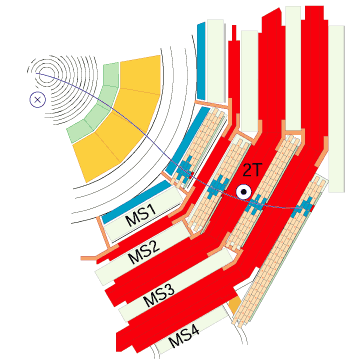
\includegraphics[width=0.4\linewidth]{figs/MCcms.png}
\end{figure}
Muons, which is considered to be stable in the CMS perspective due to its lifetime, provide clean signatures unlike hadrons.
Muon system's reconstruction efficiency is better than 98\% over the full pseudorapidity range.
Each muon station has several layers of aluminum drift tubes (DT) for the barrel region and cathode strip chambers (CSCs) for the endcap region.
The DT and CSC detectors are used to obtain a precise measurement of the 4 vector of the muons.
The DT and CSC are complemented by resistive plate chambers (RPCs), which are fast gaseous muon detectors that provide a muon trigger system. 
Large thickness of the absorber material (iron) ensures muons do not escape the detector, thereby increasing its identification efficiencys. 

Muons detected and triggered by the Muon Chamber feeds into muon reconstruction algorithms.
In reconstruction algorithms, position, direction vectors and an estimate of the muon transverse momentum are used as seeds for the track fits using the Kalman filter technique. 
The result is a collection of reco::track objects, reconstructed as "standalone muons".
For each standalone muon track, a search for tracks matching it among those reconstructed in the inner tracking system ("inner tracks" or "silicon tracks")  is performed.
The best-matching tracker track and "standalone muon" pair, based on the Kalman filter technique, gives a collection of reco::Track objects referred to as "global muons". 
A complementary approach, by considering all tracker tracks to be potential muon candidates with compatible signatures in the calorimeters and in the muon system, provides a collection of reco::Track objects referred to as "tracker muons". 

\section{Tracker of the CMS more in detail}
\begin{figure}[h!]
	\caption{Cross-section of the trackers in the CMS detector. It shows the pixels in the inner tracker for more precise vertexing and the silicon strips on the outer trackers. Silicon strips are tilted with respect to previous layers of strips. \cite{trk}}
  \label{fig:tracker}
  \centering
  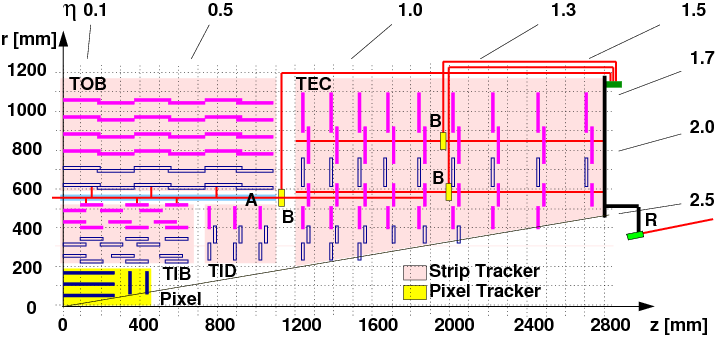
\includegraphics[width=0.9\linewidth]{figs/Tracker.png}
\end{figure}

The inner tracker is the first detector material sitting around the LHC beampipe. 
It consists of the pixel cells in the innermost part, and silicon strip sensors in the outer part of the tracker.
The inner-most tracking material consists of 3 layers of silicon pixel detectors. 
During Run 2 of 2017-2018, additional pixel layer was added for even better performance.
The square pixel detectors with high granularity are extremely radiation resistant and provide most accurate position information.
The outer layers of the tracker consist of strip sensors, which are more financially affordable.
They are of 5.8 m length, 2.6m diameter, 10 layers, and consists of 25,000 silicon strip sensors in cylindrical shape. 
The system provides analogue data from about 10 million channels. 
Each layer is oriented a slight off-angle with respect to the previous layer for 2D position measurement.

The CMS tracking system, with the magnetic field coming from the superconducting magnet, reconstruct muons, electrons and charged hadrons' tracks with high momentum resolution with efficiency better than 98\% in pseudorapidity upto 2.5.
They provide the required granularity and precision to deal with high track multiplicities.
For muons, with information from the measurements of the muon chamber, the tracking system contributes to even better resolution.

The tracker is quintessential for many physics analyses.
Its closest placement to the interaction point provides precise vertex reconstruction and measurement of the impact parameter (IP) of tracks.
The trackers' reconstruction for secondary vertices is critical for b-tagging, a method of detecting jets arising from b quark decays.
It is a frequently used tool in many CMS groups.
For instance, physicists studying Lepton Universality uses b-tagging, enabled by the tracker's good vertex reconstruction efficiency, to identify physics process involving B mesons to Kaons.
In addition, physicists use b-tagging to identify top quarks, which is another good portal for BSM physics along with the Higgs boson and mostly decay into b-jets.
The tracker's impact parameter values also play significant role in discovery of BSM physics targetting for LLPs.
LLPs IP values are starkly different from SM particles' IP values.



\section{Trigger of the CMS}
Discovery of new physics requires not only high energy, but also large statistics.
New physics, for sake of not being discovered so far, has a very small cross-section.
Large statistics is necessary to confirm existence of the small cross-section signal over standard model backgrounds.
In order to achieve the high statistics, the CMS beam crossing happens at a very high rate with bunches of protons shooted together.
CMS beam crossings occur in the CMS detector at a rate of 40 million per second (40MHz) with spacing of 25ns, while 25-50 bunch crossings are usual in CMS.
It totals at about 1 billion events occurring in the CMS detector per second. 

Proton-proton interactions are very messy and produce many tracks given its QCD nature.
However, most of the events are "not interesting" to be even considered as candidates of potentially interesting events.
These events occur too quickly to be recorded and would take up vast amounts of disk space to store, which would be wast of electronic resources. 
In order to filter and save only "interesting" events in the extreme environment, CMS employs the Trigger and Data Acquisition System. 
It selects the most interesting hundred or so events for storage and further analysis with fast electronics and resolution.
The CMS Data Acquisition System and Triggering are described below.

The first level of triggering, Level 1 (L1), is a hardware trigger.
It uses hardware processors to rapidly select or reject events based on information from the ECAL and Muon Chamber. 
The Level 1 trigger reduces the event rate from 40MHz to 100kHz.
An event passing the L1 trigger decision is transmitted to the Data Acquisition System where information from the 16M channels in the CMS subdetector systems is combined by the event builder into a single event. 
This event is then challenged by the next level of triggering.

The High Level Trigger (HLT) is a software-based trigger which performs a more sophisticated analysis of the event, including applying fast pattern recognition algorithms and event reconstruction. 
The main reduction factor for events passing the Level 1 triggering is obtained by using tracker information. 
The HLT decision reduces the event rate to about 100Hz for storage and later offline analysis. 
This corresponds to about 12 Petabytes of data to be recorded by CMS annually when it is running at design luminosity. 
The average processing time for the high level trigger is 40ms per event.
